
\section{流程控制-迴圈}

\subsection{迴圈}
\subsubsection {while}
\begin{enumerate}
	\item 講解︰JA-003:1+2+3+...+100
		\begin{enumerate}
			\item 題目說明:
			\subitem 使用 while 迴圈計算 1+2+3+...+100
			
			\item 解題思維:
			\begin{enumerate}
				\item 宣告一個初始值為零的變數sum=0,準備進行累加。
				\item 使用while迴圈,當符合while的執行條件(n<100)時,會重複執行累加計算,累加完之後會更新n的值,當n不滿足執行條件時,結束迴圈。
				
			\end{enumerate}
				\begin{cppcode}
				#include <iostream>
				
				using namespace std;
				
				int main()
				{
					int n=1, sum=0;
					while (n<=100) {
						sum += n; // 累加
						n++; // 更新n
					}
					cout << sum;
					return 0;
				}
				
			\end{cppcode}
		\end{enumerate}
		
	\item 練習:JA-004︰1+3+5+...+99
		\begin{enumerate}
			\item 題目說明:
			\subitem 使用 while 迴圈計算 1+3+5+...+99
			
			\item 解題思維:
			\subitem 使用while迴圈進行累加,只要(n<100)就對sum進行累加,每次累加完後,n加上2。
\begin{comment}			
			\item 程式碼:
			\begin{cppcode}
				#include <iostream>
				
				using namespace std;
				
				int main()
				{
					int n=1, sum=0;
					while (n<100) {
						sum += n;
						n += 2;
					}
					cout << sum;
					return 0;
				}
				
			\end{cppcode}
\end{comment}
		\end{enumerate}
	
\end{enumerate}

\subsubsection {for}
\begin{enumerate}
	\item 講解︰JA-005:1+2+3+...+100
		\begin{enumerate}
			\item 題目說明:
			\subitem 使用 for 迴圈計算 1+2+3+...+100
			
			\item 解題思維:
			\subitem for迴圈的用法是for(起始值; 條件式; 更新值),本題的for迴圈寫法如下:
			\begin{inside}
				for (int i=1; i<=100; i++) sum += i;
			\end{inside}
			意思是:i的起始值是1,當i<=100這個條件成立時的時候,會重複執行累加(sum += i;),並在累加完後更新i的值(i++)。此迴圈總共回會複執行100次累加的計算。
			
			\item 程式碼:
			\begin{cppcode}
				#include <iostream>
				
				using namespace std;
				
				int main()
				{
					int sum=0;
					for (int i=1; i<=100; i++) sum += i;
					cout << sum;
					return 0;
				}
				
			\end{cppcode}
		\end{enumerate}
	
	\item 練習︰JA-006:1+3+5+...+99
		\begin{enumerate}
			\item 題目說明:
			\subitem 使用 for 迴圈計算 1+3+5+...+99
			
			\item 解題思維:
			\subitem 使用for迴圈進行累加,只要(n<100)就對sum進行累加,n每次更新都加2。
\begin{comment}			
			\item 程式碼:
			\begin{cppcode}
			#include <iostream>
			
			using namespace std;
			
			int main()
			{
				int sum=0;
				for (int i=1; i<100; i+=2) sum += i;
				cout << sum;
				return 0;
			}
				
			\end{cppcode}
\end{comment}
		\end{enumerate}
	
\end{enumerate}

\subsubsection {應用題}
\begin{enumerate}
	\item 講解︰JT-04:印三角形函數
		\begin{enumerate}
			\item 題目說明:
			\subitem 輸入N,印出N列的星號(*),其中第I列有I個星,如執行範例所示。
			\subitem 範例輸入:5
			\subitem 範例輸出:
				\begin{figure}[H]
					\centering
					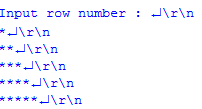
\includegraphics{fig/JT04fig}
				\end{figure}
			
			\item 解題思維:
			\subitem 
				這題需要使用雙重for迴圈。第一個迴圈計算現在要印第幾列,第二個迴圈計算要印幾個星。
			\item 程式碼:
			\begin{cppcode}
				#include <stdio.h>
				
				int main()
				{
					int n, i, j;
					printf("Input row number : \n");
					scanf("%d", &n);
					for (i=1; i<=n; i++) { // 迴圈1:第i列
						for(j=0; j<i; j++) { // 迴圈2:印i個星
							printf("*");
						}
						printf("\n");
					}
					return 0;
				}
					
			\end{cppcode}
		\end{enumerate}

	\item 練習︰JP-010-2:印倒三角形(無空白)
		\begin{enumerate}
			\item 題目說明:
			\subitem 輸入正整數n<=20,輸出一個n層的倒三角形。
			\subitem 範例輸入:5
			\subitem 範例輸出:
			\begin{figure}[H]
				\centering
				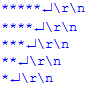
\includegraphics{fig/JP010fig}
			\end{figure}
			\item 解題思維:
			\subitem 印倒三角形時,第一列有n個星,下一列有n-1個星,以此列推,每換一列就少一個星,所以這題是要使用for迴圈來倒數。
\begin{comment}
			\item 程式碼:
			\begin{cppcode}
			#include <cstdio>
			
			int main()
			{
				int n, i, j;
				scanf("%d", &n);
				for (i=n; i>0; i--) { // 迴圈1:計算此列有i個星
					for(j=i; j>0; j--) { // 迴圈2:印出i個星
						printf("*");
					}
					printf("\n");
				}
				return 0;
			}
				
			\end{cppcode}
\end{comment}
		\end{enumerate}
	
	\item 挑戰︰JT-40印等腰三角形
		\begin{enumerate}
			\item 題目說明:
			\subitem 輸入N,印出一個N列的等腰三角形,其中第I列有2*I-1個\#,如程式範例結果所示。
			\subitem 範例輸入:5
			\subitem 範例輸出:
			\begin{figure}[H]
				\centering
				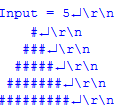
\includegraphics{fig/JT40fig}
			\end{figure}
			
			\item 解題思維:
			\begin{enumerate}
				\item 因為要印出N列,所以先寫一個執行N次的for迴圈,用變數row來計算現在是第幾列。
				\item 第row列要印出(n-row)個``空白",及(2*row-1)個``\#",所以分別用兩個for迴圈印``空白"及``\#"。
			\end{enumerate}
\begin{comment}			
			\item 程式碼:
			\begin{cppcode}
				#include <stdio.h>
				
				int main()
				{
					int i, row, n;
					scanf("%d", &n);
					printf("Input = %d\n", n);
					for (row=1; row<=n; row++) {
						for (i=0; i<n-row; i++) printf(" ");
						for (i=0; i<2*row-1; i++) printf("#");
						printf("\n");
					}
					return 0;
				}
				
			\end{cppcode}
\end{comment}
		\end{enumerate}

\end{enumerate}

%\subsubsection {do while {\color{blue}(若有多餘時間)}}

